% Description du contenu du rapport à rendre pour l'UF temps réel en 4AE et 4IR
% Auteur : P.-E. Hladik
% Institut : INSA de Toulouse

\documentclass[11pt, a4paper]{paper}
\usepackage{a4wide,color}

\usepackage[utf8]{inputenc}
\usepackage[T1]{fontenc}
\usepackage[french]{babel}

\usepackage{graphicx}
\usepackage{amssymb}
\usepackage{hyperref}

\usepackage{amstext}
\usepackage{amsmath}

\usepackage[dvipsnames]{xcolor}

\usepackage{placeins}

\newcounter{cptreq}


\usepackage{framed}


\title{{\Huge Rapport de projet De Stijl 2.0}\\
{\large version \today}\\
---\\
}
\author{{Laura Bouzereau (conception, vidéo, robot, mission, rédaction du compte-rendu)}\\
{Constance Gay (robot, mission, rédaction du compte-rendu)}\\
{Louis Jean (conception, robot, intégration)}\\
}

\begin{document}

%%%%%%%%%%%%%%
% PAGE DE GARDE
\maketitle

%%%%%%%%%%%%%%
% DEBUT DU RAPPORT
\newpage




%%%%%%%%%%%%%%
% CONCEPTION
\section{Conception}

% VUE GENERAL DU SYSTEME
\subsection{Diagramme fonctionnel général}

{Ci-dessous est le diagramme fonctionnel de notre système, faisant référence aux différents threads que nous détaillerons plus bas.}

\begin{figure}[htbp]
\begin{center}
{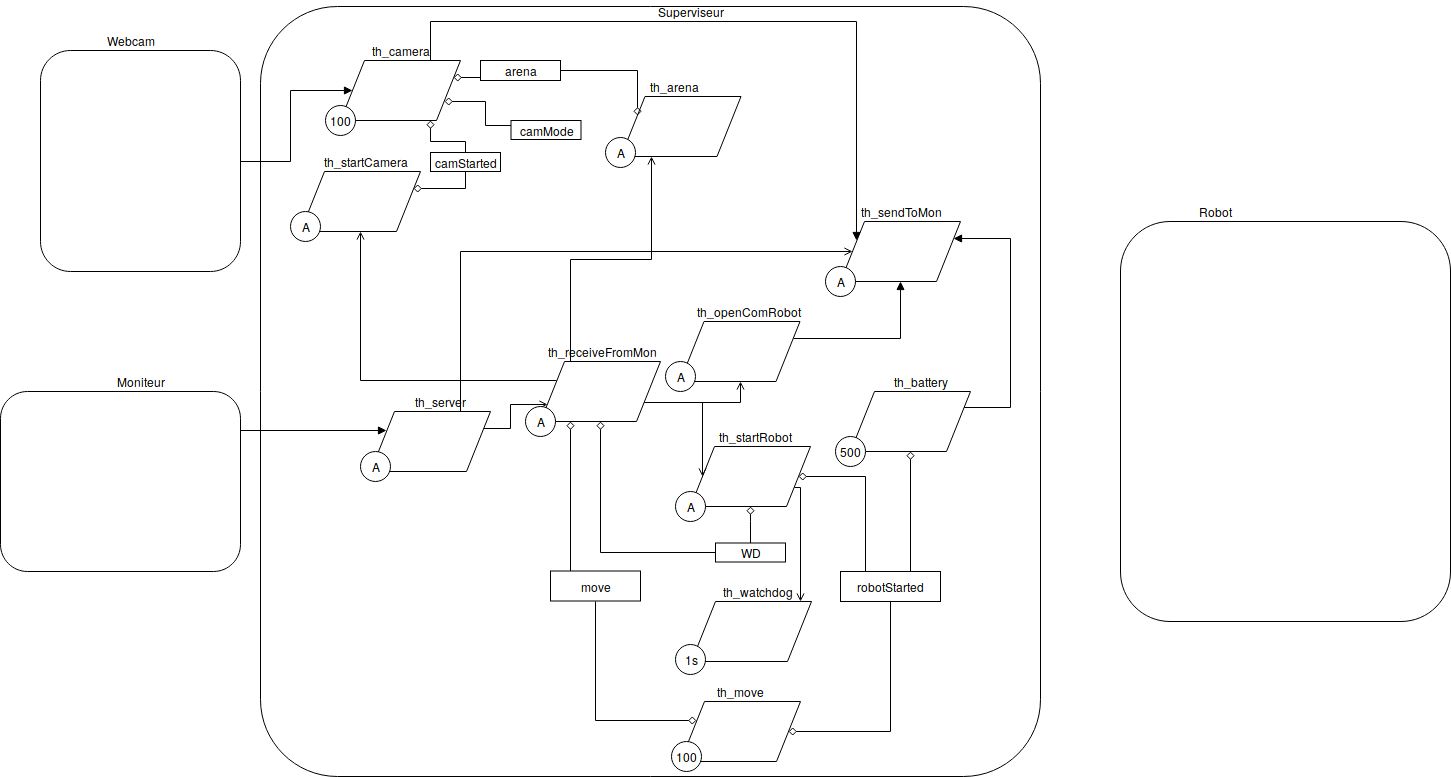
\includegraphics[scale=.3]{./dossier_conception/conception_generale}}
{\caption{Diagramme fonctionnel du système}}
\end{center}
\label{fig:diag_fonc_gen}
\end{figure}
\FloatBarrier

% DIAGRAMME FONCTIONNEL GT MONITEUR
\subsection{Groupe de threads gestion du moniteur}


% DIAGRAMME FONCTIONNEL GT MONITEUR
\subsubsection{Diagramme fonctionnel du groupe gestion du moniteur}

{Le moniteur a pour fonction de gérer les communications avec le robot, de récupérer les informations (niveau de batterie, perte de connexion...) et d'envoyer des ordres permettant d'effectuer les différentes actions (déplacer robot, allumer camera...).}

\begin{figure}[htbp]
\label{fig:diag_fonc_moniteur}
\begin{center}
{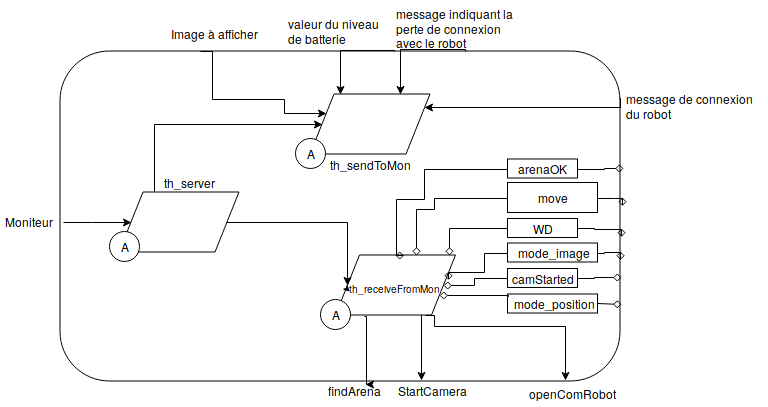
\includegraphics[scale=.4]{./dossier_conception/diag_fonc_moniteur}}
{\caption{Diagramme fonctionnel du groupe de threads gestion du moniteur}}
\end{center}
\end{figure}
\FloatBarrier

% DESCRIPTION THREADS GT MONITEUR
\subsubsection{Description des threads  du groupe gestion du moniteur}

\begin{table}[htp]
\caption{Description des threads du groupe {\tt th\_group\_gestion\_moniteur}}
\begin{center}
\begin{tabular}{|p{4cm}|p{7.5cm}|p{2cm}|}
\hline
\bf Nom du thread &	\bf Rôle &	\bf Priorité \\
\hline
\hline
\color{blue}th\_server	& \color{blue}S'occupe de créer un server où le moniteur peut se connecter & \color{blue}30\\
\hline
\color{blue}th\_receiveFromMon &	\color{blue}Gère la reception des messages en provenance du moniteur et l'action demandée est effectuée &	\color{blue}25\\
\hline
\color{blue}th\_sentToMon	& \color{blue}Gère l'envoi des messages du robot au moniteur & \color{blue}23\\
\hline
\end{tabular}
\end{center}
\label{tab:gt_moniteur}
\end{table}%

% DIAGRAMMES D'ACTIVITE GT MONITEUR
\subsubsection{Diagrammes d'activité  du groupe gestion du moniteur}
%{\color{red}Décrivez le comportement de chacun de vos threads avec des diagrammes d'activité. Apportez les explications qui vous semblent nécessaires pour comprendre votre conception. A titre d'exemple les diagrammes fonctionnels tirés du document de conception sont remis.}

{Le thread th\_server ouvre une connexion pour le moniteur. Quand ce dernier essaye de se connecter en tant que client, sa demande est acceptée et notifie le moniteur. } 

\begin{figure}[htbp]
\label{fig:act_envoyer}
\begin{center}
{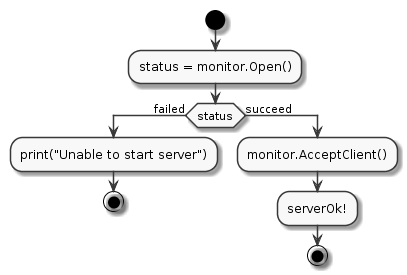
\includegraphics[scale=.3]{./figures-pdf/th_server}}
{\caption{Diagramme d'activité du thread {\tt th\_server}}}
\end{center}
\end{figure}
\FloatBarrier

{Le thread th\_sendToMon a pour fonction d'attendre des messages destinés au moniteur et de les récupérer à leur arrivée. }

\begin{figure}[htbp]
\label{fig:act_envoyer}
\begin{center}
{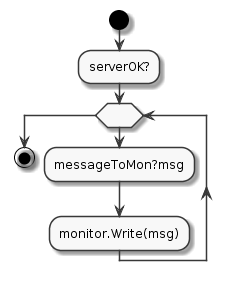
\includegraphics[scale=.3]{./figures-pdf/th_sendToMon}}
{\caption{Diagramme d'activité du thread {\tt th\_sendToMon}}}
\end{center}
\end{figure}
\FloatBarrier

{ Le thread th\_receiveFromMon reçoit des messages provenant du moniteur indiquant les actions à effectuer par le biais de messages prédéfinis. Les actions pouvant être demandées sont: ouverture de la communication, démarrage avec et sans watchdog, ouverture de la caméra, déplacement du robot, changement du mode d'acquisition de la caméra et affichage d'une image. }

\begin{figure}[htp]
\label{fig:act_communiquer}
\begin{center}
{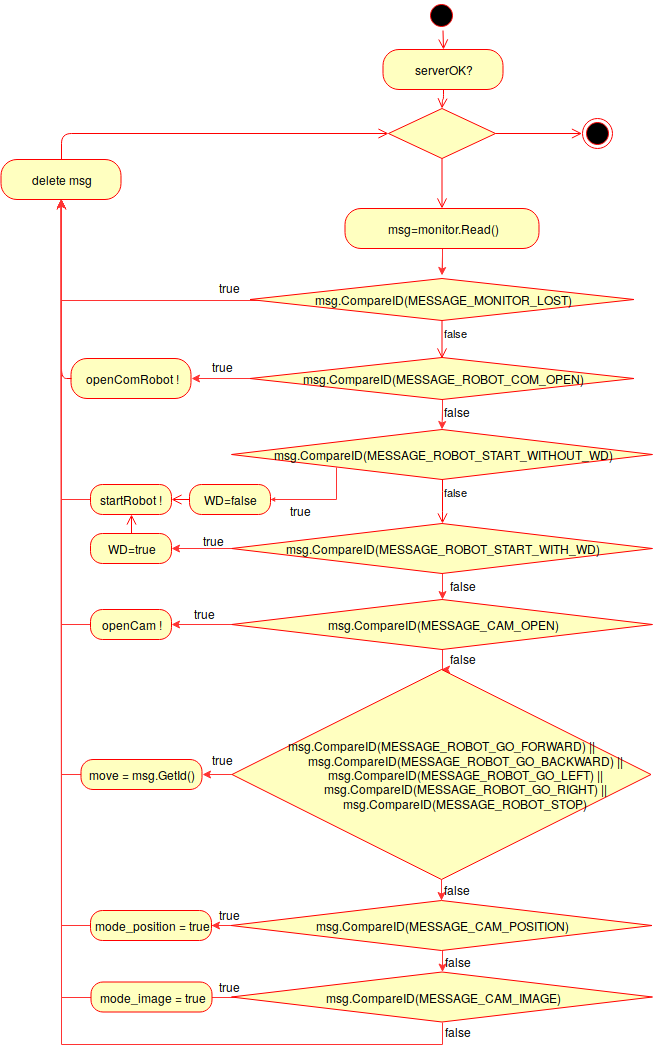
\includegraphics[scale=.4]{./dossier_conception/th_receiveFromMon.png}}
{\caption{Diagramme d'activité du thread {\tt th\_receiveFromMon}}}
\end{center}
\end{figure}
\FloatBarrier

% DIAGRAMME FONCTIONNEL GT VISION
\subsection{Groupe de threads vision}

% DIAGRAMME FONCTIONNEL GT VISION
\subsubsection{Diagramme fonctionnel du groupe vision}

{Le groupe vision contient tout ce qui concerne la caméra et l'arène. Il va permettre d'allumer la caméra, de capturer des images dans deux modes différents (position et image) et de chercher une arène sur une photo.}

\begin{figure}[htp]
\label{fig:act_communiquer}
\begin{center}
{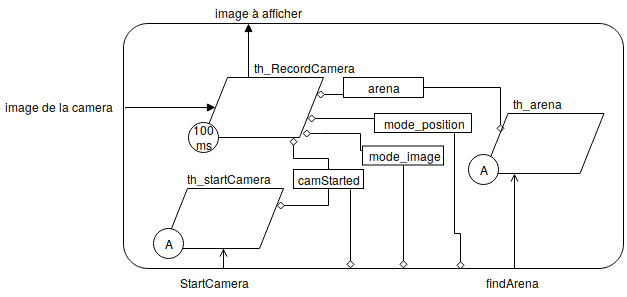
\includegraphics[scale=.4]{./dossier_conception/diag_fonc_vision.png}}
{\caption{Diagramme fonctionnel du groupe de threads gestion de la vision}}
\end{center}
\end{figure}

% DESCRIPTION THREADS GT VISION
\subsubsection{Description des threads du groupe vision}

\begin{table}[htp]
\caption{Description des threads du groupe {\tt th\_group\_vision}}
\begin{center}
\begin{tabular}{|p{3cm}|p{8.5cm}|p{2cm}|}
\hline
\bf Nom du thread &	\bf Rôle &	\bf Priorité \\
\hline
\hline
\color{blue}th\_startCamera &	\color{blue}Démarre la caméra &	\color{blue}18\\
\hline
\color{blue}th\_arena &	\color{blue}Cherche une arène sur une image et la sauvegarde si elle est trouvée (demande confirmation à l'utilisateur) &	\color{blue}17\\
\hline
\color{blue}th\_RecordCamera &	\color{blue}Renvoie des photos selon le mode (position ou image) &	\color{blue}16\\
\hline
\end{tabular}
\end{center}
\label{tab:gt_moniteur}
\end{table}%
\FloatBarrier

% DIAGRAMMES D'ACTIVITE GT VISION
\subsubsection{Diagrammes d'activité du groupe vision}
{Le thread th\_startCamera reçoit un message du moniteur, allume la caméra et notifie le moniteur en cas d'échec.}

\begin{figure}[htbp]
\label{fig:act_envoyer}
\begin{center}
{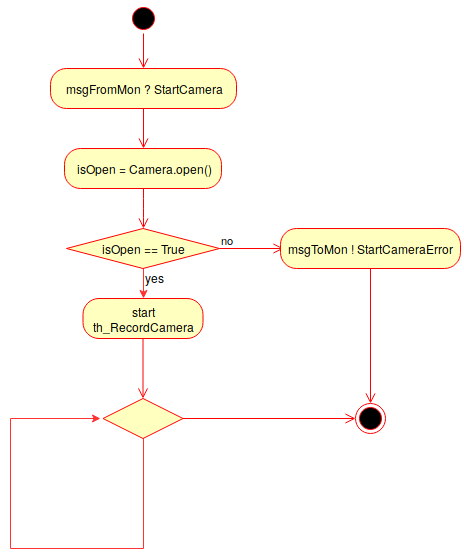
\includegraphics[scale=.3]{./dossier_conception/th_startCamera}}
{\caption{Diagramme d'activité du thread {\tt th\_startCamera}}}
\end{center}
\end{figure}
\FloatBarrier

{Le thread th\_arena démarre lorsque que l'utilisateur appuie sur un bouton. Ce thread reçoit alors l'ordre de chercher l'arène sur une image. Le thread va donc mettre en pause la caméra, prendre une photo et chercher l'arène sur cette photo. S'il la trouve, il notifie le moniteur qui va demander une confirmation de l'utilisateur. Si l'utilisateur confirme que l'arène est bien sur la photo, le thread th\_arena va enregistrer l'image et s'arrêter. }

\begin{figure}[htbp]
\label{fig:act_envoyer}
\begin{center}
{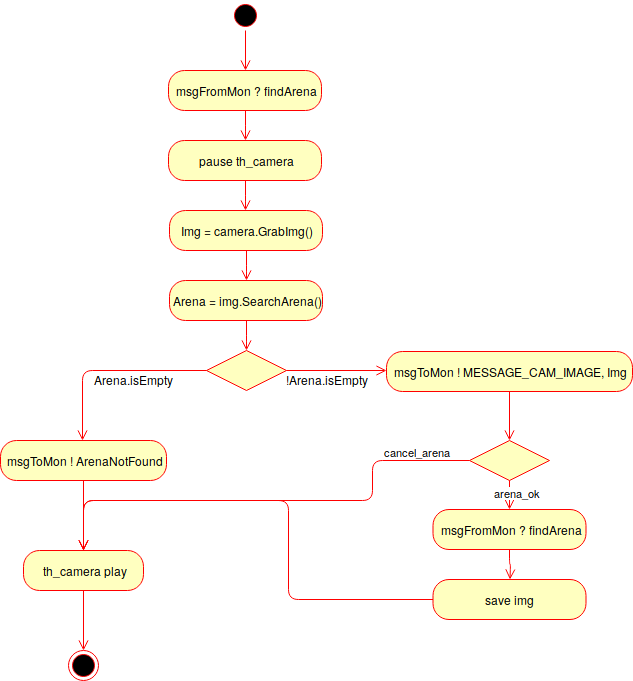
\includegraphics[scale=.3]{./dossier_conception/th_arena}}
{\caption{Diagramme d'activité du thread {\tt th\_arena}}}
\end{center}
\end{figure}
\FloatBarrier

{Le thread th\_RecordCamera gère la caméra périodiquement (100ms). Il permet de lancer la caméra dans deux modes différents. Le premier est le mode position qui permet de chercher un ou plusieurs robot(s) dans l'arène et de renvoyer sa position. Le deuxième mode est le mode image qui prend des photos et les renvoie au moniteur. Le thread peut également être mis en pause, notamment par le thread th\_arena.}

\begin{figure}[htbp]
\label{fig:act_envoyer}
\begin{center}
{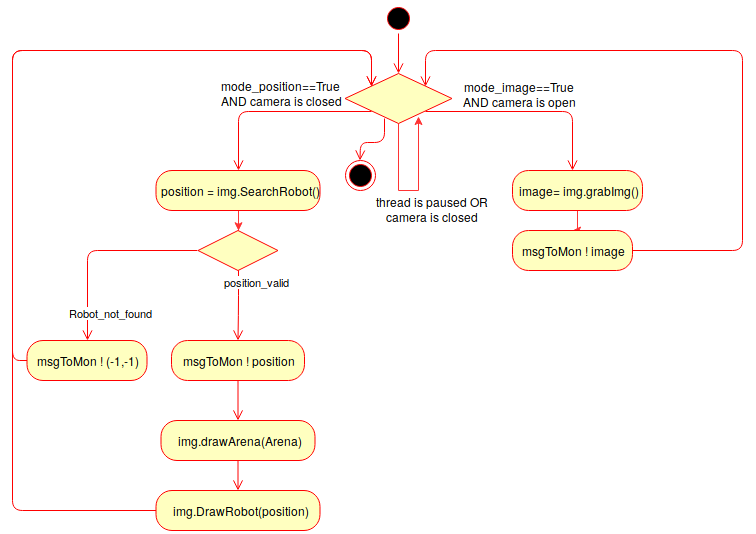
\includegraphics[scale=.3]{./dossier_conception/th_RecordCamera}}
{\caption{Diagramme d'activité du thread {\tt th\_RecordCamera}}}
\end{center}
\end{figure}
\FloatBarrier


% DIAGRAMME FONCTIONNEL GT ROBOT
\subsection{Groupe de threads gestion du robot}

% DIAGRAMME FONCTIONNEL GT ROBOT
\subsubsection{Diagramme fonctionnel du groupe gestion robot}
{Le groupe de gestion du robot permet d'effectuer les différentes actions du robot, notamment son déplacement, l'ouverture de ses communications, contrôler son niveau de batterie et surveiller sa connexion avec le moniteur.}

\begin{figure}[htp]
\label{fig:act_communiquer}
\begin{center}
{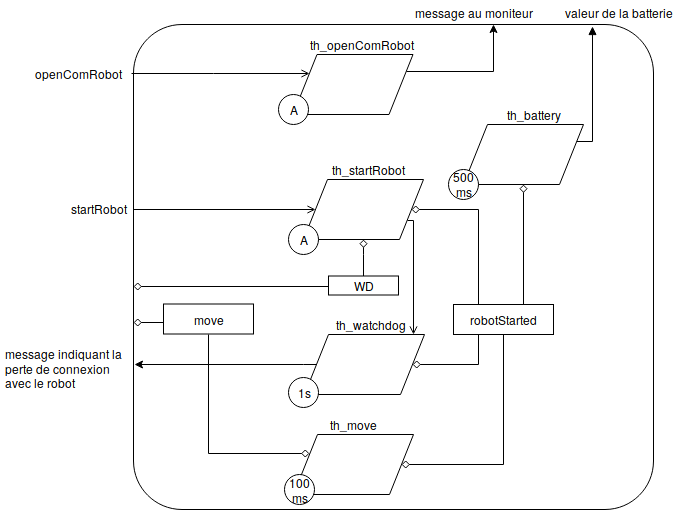
\includegraphics[scale=.4]{./dossier_conception/diag_fonc_robot.png}}
{\caption{Diagramme fonctionnel du groupe de threads gestion du robot}}
\end{center}
\end{figure}

% DESCRIPTION THREADS GT ROBOT
\subsubsection{Description des threads du groupe gestion robot}

\begin{table}[htp]
\caption{Description des threads du groupe {\tt th\_group\_gestion\_robot}}
\begin{center}
\begin{tabular}{|p{3cm}|p{8.5cm}|p{2cm}|}
\hline
\bf Nom du thread &	\bf Rôle &	\bf Priorité \\
\hline
\hline
\color{blue}th\_watchdog	& \color{blue}Vérifie la connexion entre le moniteur et le robot & \color{blue}22\\
\hline
\color{blue}th\_openComRobot	& \color{blue}Démarre la communication avec le robot & \color{blue}20\\
\hline
\color{blue}th\_startRobot	& \color{blue}Démarre le robot & \color{blue}20\\
\hline
\color{blue}th\_move	& \color{blue}Permet de déplacer le robot & \color{blue}20\\
\hline
\color{blue}th\_battery	& \color{blue}Récupère le niveau de batterie du robot & \color{blue}15\\
\hline
\end{tabular}
\end{center}
\label{tab:gt_moniteur}
\end{table}%
\FloatBarrier

% DIAGRAMMES D'ACTIVITE GT ROBOT
\subsubsection{Diagrammes d'activité du groupe robot}
{Nous n'allons pas décrire les threads th\_openComRobot et th\_move car aucun modification n'a été appliquée. En ce qui concerne le thread th\_startRobot nous n'avons fait qu'une légère modification afin de choisir le mode de démarrage, c'est-à-dire avec ou sans watchdog.}\\ \\

{Le thread th\_watchdog se lance si le robot est démarré en mode watchdog. Ce thread envoie des messages périodiquement (toutes les secondes) au robot et si 3 messages de suite sont ne sont pas acquittés, le système entier (moniteur, robot...) se réinitialisera puis s'éteindra.}

\begin{figure}[htbp]
\label{fig:act_envoyer}
\begin{center}
{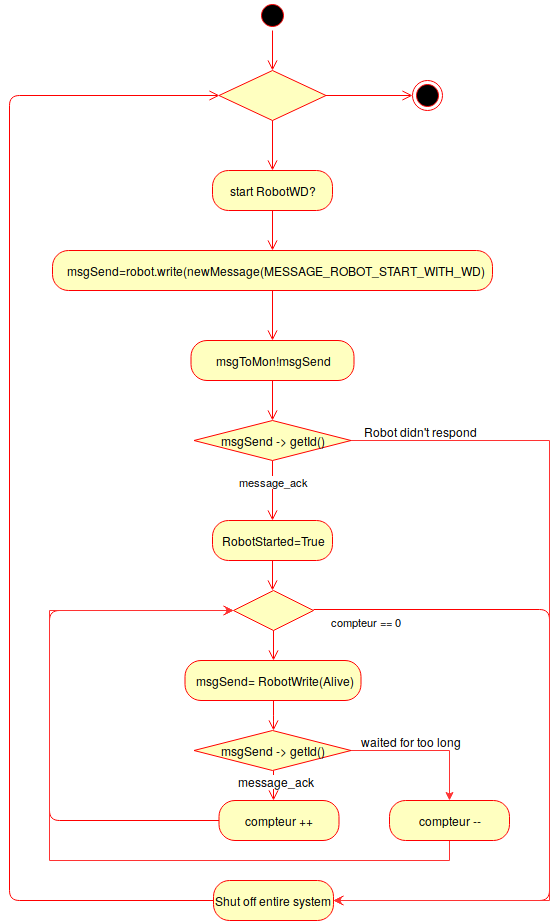
\includegraphics[scale=.3]{./dossier_conception/th_watchdog}}
{\caption{Diagramme d'activité du thread {\tt th\_watchdog}}}
\end{center}
\end{figure}
\FloatBarrier

{Le thread th\_battery permet d'envoyer un message toutes les 500ms au moniteur contenant le niveau de batterie du robot.}

\begin{figure}[htbp]
\label{fig:act_envoyer}
\begin{center}
{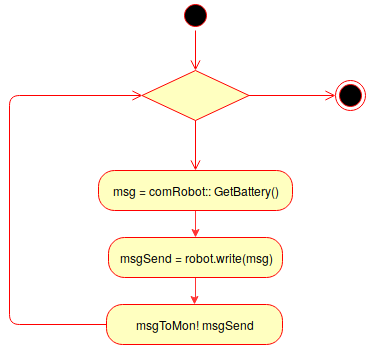
\includegraphics[scale=.3]{./dossier_conception/th_battery}}
{\caption{Diagramme d'activité du thread {\tt th\_battery}}}
\end{center}
\end{figure}
\FloatBarrier

%%%%%%%%%%%%%%%
% ANALYSE ET VALIDATION
\section{Analyse et validation de la conception}

{\color{black}
\stepcounter{cptreq}
\subsection{Fonctionnalité \thecptreq *}

\paragraph{Description :} Le lancement du serveur doit être réalisé au démarrage du superviseur. En cas d'échec du démarrage du serveur, un message textuel doit être  affiché sur la console de lancement de l'application. Ce message doit signaler le problème et le superviseur doit s'arrêter.

}
%%%
{\color{black}
\stepcounter{cptreq}
\subsection{Fonctionnalité \thecptreq *}

\paragraph{Description :} La connexion entre le moniteur et le superviseur (via le socket) doit être établie suite à la demande de connexion de l'utilisateur.

%%%
{\color{black}
\stepcounter{cptreq}
\subsection{Fonctionnalité \thecptreq *}

\paragraph{Description :} Tous les messages envoyés depuis le moniteur doivent être réceptionnés par le superviseur.

%%%
\stepcounter{cptreq}
\subsection{Fonctionnalité \thecptreq *}

\paragraph{Description :} L'application superviseur doit être capable d'envoyer les messages au moniteur (via le serveur) avec un délai d'au plus 10~ms.

%%%
\stepcounter{cptreq}
\subsection{Fonctionnalité \thecptreq *}

\paragraph{Description :} Le superviseur doit détecter la perte de communication avec le moniteur. En cas de perte de la communication un message doit être affiché sur la console de lancement du superviseur.

%%%
\stepcounter{cptreq}
\subsection{Fonctionnalité \thecptreq *}

\paragraph{Description :} En cas de perte de communication entre le superviseur et moniteur, il faut stopper le robot,  la communication avec le robot, fermer le serveur et déconnecter la caméra afin de revenir dans le même état qu'au démarrage du superviseur.

%%%
{\color{black}
\stepcounter{cptreq}
\subsection{Fonctionnalité \thecptreq *}

\paragraph{Description :} Dès que la communication avec le moniteur est en place, la communication entre le superviseur et le robot doit être ouverte. Si la communication est active, il faut envoyer un message d'acquittement au moniteur. En cas d'échec, un message le signalant est renvoyé au moniteur.

}
%%%
\stepcounter{cptreq}
\subsection{Fonctionnalité \thecptreq }

\paragraph{Description :} La communication entre le robot et le superviseur doit être surveillée par un mécanisme de compteur afin de détecter une perte du médium de communication.

\paragraph{\color{black}Réalisation :}  {\color{black} Nous avons traité cette fonctionnalité par le développement d'un thread périodique th\_watchdog. Celui-ci indique au robot qu'il doit démarrer en mode watchdog, et attend que celui-ci confirme son démarrage. Ensuite, le moniteur envoit un message périodiquement au robot (toutes les 500ms). Dans notre diagramme, nous avons décidé d'incrémenter notre compteur à chaque réception de message et décrementer à chaque perte. Lors de la réalisation, nous avons plutôt choisi de déclarer la connexion comme perdue uniquement si trois messages de suite n'ont pas de réponse. Le watchdog est complètement rechargé si la communication est rétablie. Si la connexion est perdue le système entier s'éteint, comme décrit ci-dessous avec la fonctionnalité 9. }

%%%
\stepcounter{cptreq}
\subsection{Fonctionnalité \thecptreq }

\paragraph{Description :} Lorsque la communication entre le robot et le superviseur est perdue, un message spécifique doit être envoyé au moniteur. Le système doit fermer la communication entre le robot et le superviseur et se remettre dans un état initial permettant de relancer la communication.

\paragraph{\color{black}Réalisation :}  {\color{black} Cette fonctionnalité a été traitée à la suite de la précédente dans le thread th\_watchdog: si une perte de connexion est détectée, un message est affiché sur la console, un message MESSAGE\_ANSWER\_ROBOT\_TIMEOUT est envoyé au moniteur, la communication avec le robot est fermée et la variable RobotStarted est remise à 0. Le système est donc complètement réinitialisé.}

%%%
{\color{black}
\stepcounter{cptreq}
\subsection{Fonctionnalité \thecptreq *}

\paragraph{Description :} Lorsque l'utilisateur demande, via le moniteur, le démarrage sans watchdog, le robot doit démarrer dans ce mode. En cas de succès, un message d'acquittement est retourné au moniteur. En cas d'échec, un message indiquant l'échec est transmis au moniteur.

}
%%%
\stepcounter{cptreq}
\subsection{Fonctionnalité \thecptreq}

\paragraph{Description :} Lorsque l'utilisateur demande, via le moniteur, le démarrage avec watchdog, le robot doit démarrer dans ce mode. Un message d'acquittement est retourné au moniteur. En cas d'échec, un message indiquant l'échec est transmis au moniteur.

Une fois le démarrage effectué, le robot doit rester vivant en envoyant régulièrement le message de rechargement du watchdog.

\paragraph{\color{black}Réalisation :}  {\color{black} Cette fonctionnalité est implémentée dans le thread th\_startRobot. Une variable partagée (WD) nous permet de stocker le mode de connexion. Dans ce thread, un message est envoyé au moniteur lui indiquant dans quel mode la connexion a été établie.}

%%%
{\color{black}
\stepcounter{cptreq}
\subsection{Fonctionnalité \thecptreq *}

\paragraph{Description :} Lorsque qu'un ordre de mouvement est reçu par le superviseur, le robot doit réaliser ce déplacement en moins de 100~ms.

}
%%%
\stepcounter{cptreq}
\subsection{Fonctionnalité \thecptreq}

\paragraph{Description :} Le niveau de la batterie du robot doit être mis à jour toutes les 500~ms sur le moniteur.

\paragraph{\color{black}Réalisation :}  {\color{black} Nous avons implémenté cette fonctionnalité avec le thread th\_battery qui renvoie toutes les 500ms le niveau de batterie du robot au moniteur.}
%%%
\stepcounter{cptreq}
\subsection{Fonctionnalité \thecptreq}

\paragraph{Description :} La caméra doit être démarrée suite à une demande provenant du moniteur. Si l'ouverture de la  caméra a échoué, il faut envoyer un message au moniteur.

\paragraph{\color{black}Réalisation :}  {\color{black} Le thread th\_StartCamera est lancé suite à la demande de l'utilisateur via le moniteur. Le moniteur envoie une message à ce thread ce qui entrainera le démarrage de la caméra. Si ce démarrage échoue, un message est renvoyé au moniteur (StartCameraError) et le thread se termine. Si le démarrage fonctionne le thread th\_RecordCamera est démarré.}
%%%
\stepcounter{cptreq}
\subsection{Fonctionnalité \thecptreq}

\paragraph{Description :} Dès que la caméra est ouverte, une image doit être envoyée au moniteur toutes les 100 ms.

\paragraph{\color{black}Réalisation :}  {\color{black} Le thread th\_RecordCamera est lancé avec une période de 100ms. Il vérifie que la caméra est toujours ouverte et le mode d'acquisition. Si la variable partagée mode\_image vaut true, alors une image est renvoyée au moniteur à chaque itération.}
%%%
\stepcounter{cptreq}
\subsection{Fonctionnalité \thecptreq}

\paragraph{Description :} La caméra doit être fermée suite à une demande provenant du moniteur. Un message doit être envoyé au moniteur pour signifier l'acquittement de la demande. L'envoi périodique des images doit alors être stoppé.

\paragraph{\color{black}Réalisation :}  {\color{black} Si une demande de fermeture de caméra est faite par le moniteur (MESSAGE\_CAMERA\_CLOSE), alors la caméra sera fermée par le thread th\_ReceiveFromMon. Ainsi, le thread th\_RecordCamera détectera que la caméra a été fermée et cessera d'enregistrer des images. Nous ne renvoyons pas d'acquittement au moniteur.  }
%%%
\stepcounter{cptreq}
\subsection{Fonctionnalité \thecptreq}

\paragraph{Description :} Suite à une demande de recherche de l'arène, le superviseur doit stopper l'envoi périodique des images, faire la recherche de l'arène et renvoyer une image sur laquelle est dessinée cette arène. Si aucune arène n'est trouvée un message d'échec est envoyé.\\

L'utilisateur doit ensuite valider visuellement via le moniteur si l'arène a bien été trouvée. L'utilisateur peut :
\begin{itemize}
	\item valider l'arène : dans ce cas, le superviseur doit sauvegarder l'arène trouvée (pour l'utiliser ultérieurement) puis retourner dans son mode d'envoi périodique des images en ajoutant à l'image l'arène dessinée.
 	\item annuler la recherche : dans ce cas, le superviseur doit simplement retourner dans son mode d'envoi périodique des images et invalider la recherche.
\end{itemize}

\paragraph{\color{black}Réalisation :}  {\color{black} Lorsqu'une demande de recherche d'arène arrive du moniteur, le thread th\_arena démarre. Il prend ensuite le sémaphore sem\_recordCamera, afin de mettre en pause le thread th\_RecordCamera jusqu'à la libération du sémaphore. L'envoi périodique des images est donc stoppé.\\
Le thread th\_arena va ensuite chercher l'arène. S'il la trouve, l'image contenant l'arène sera envoyée au moniteur MESSAGE\_CAM\_IMAGE. Sinon le moniteur sera notifié de l'échec.\\
L'utilisateur doit ensuite confirmer la validité de l'image. Si c'est le cas, le moniteur enverra le message MESSAGE\_CAM\_ARENA\_CONFIRM et l'image sera enregistrée. Sinon le moniteur enverra le message MESSAGE\_CAM\_ARENA\_INFIRM. \\
Après cela, le semaphore sem\_recordCamera est relaché pour libérer le thread th\_RecordCamera.}

%%%
\stepcounter{cptreq}
\subsection{Fonctionnalité \thecptreq}

\paragraph{Description :} Suite à une demande de l'utilisateur de calculer la position du robot, le superviseur doit calculer cette position, dessiner sur l'image le résultat et envoyer un message au moniteur avec la position toutes les 100~ms. Si le robot n'a pas été trouvé, un message de position est envoyé avec une position (-1,-1).

\paragraph{\color{black}Réalisation :}  {\color{black} La gestion du mode d'acquisition (image ou position) est géré par la variable partagées mode\_image. Cette variable est passée à true dans le cas où le moniteur envoie MESSAGE\_CAM\_IMAGE et false avec le message MESSAGE\_CAM\_POSITION. A chaque itération, th\_RecordCamera vérifie le mode afin d'effectuer les actions correspondantes. Le mode par défaut est le mode image (détaillé ci-dessus).\\ \\
Le mode position récupère une image , dessine l'arène précédemment enregistrée et cherche le(s) robot(s) présents dans l'arène. L'image ainsi dessinée est ensuite renvoyée au moniteur. Ainsi, les positions ne sont pas renvoyées, il n'y a pas d'envoie de (-1,-1) en cas d'échec. En effet, dans le cas où aucun robot n'est détecté, rien n'est dessiné. Cette fonctionnalité n'a pas pu être testée.}
\stepcounter{cptreq}
\subsection{Fonctionnalité \thecptreq}

\paragraph{Description :} Suite à une demande de l'utilisateur d'arrêter le calcul de la position du robot, le superviseur doit rebasculer dans un mode d'envoi de l'image sans le calcul de la position.

\paragraph{\color{black}Réalisation :}  {\color{black} Comme décrit dans la fonctionnalité précédente, le mode de prise d'image est testée à chaque itération du thread th\_RecordCamera. Si l'utilisateur le change, ce changement sera pris en compte grâce à la variable mode\_image. }


%%%%%%%%%%%%%%%%%%%
% TRANSFORMATION AADL2XENO
\section{Transformation AADL vers Xenomai}
 
 % THREAD
\subsection{Thread}
% INSTANCIATION THREAD
\subsubsection{Instanciation et démarrage}
 {\color{blue} Expliquer comment vous implémentez sous Xenomai l'instanciation et le démarrage d'un  thread AADL.}
 
 {\color{black} {Chaque thread a été implémenté par un {\tt RT\_TASK} déclarés dans le fichier {\tt tasks.h}. La création de la tâche se fait à l'aide du service {\tt rt\_task\_create} et son démarrage à l'aide de {\tt rt\_task\_start}. Toutes les tâches sont créées dans la méthode {\tt init} de {\tt tasks.cpp} et démarrées dans la méthode {\tt run}.

Par exemple, la tâche {\tt th\_server} est déclarée ligne 73 dans le fichier {\tt tasks.h}
\begin{verbatim}
  RT_TASK th_server;
\end{verbatim}
 il est créé ligne 102 de {\tt tasks.cpp} lors de l'appel de
\begin{verbatim}
  rt_task_create(&th_server, "th_server", 0, PRIORITY_TSERVER, 0)
\end{verbatim}
et son démarrage est effectué ligne 146 avec
\begin{verbatim}
  rt_task_start(&th_server, (void(*)(void*)) & Tasks::ServerTask, this)
\end{verbatim}
}

% CODE THREAD
\subsubsection{Code à exécuter}
 {\color{blue} Comment se fait le lien sous Xenomai entre le thread et le traitement à exécuter.}\\
 
 {\color{black} La fonction suivante permet de faire the lien entre un thread et son traitement}
\begin{verbatim}
  int rt_task_start(RT_TASK * task, void(*entry)(void*cookie),void*cookie);
\end{verbatim}
 

% PRIORITE THREAD
\subsubsection{Niveau de priorités}
 {\color{blue} Expliquer comment vous fixez sous Xenomai le niveau de priorité d'un thread AADL.}\\
 
{\color{black} Nous avons défini les priorités lors de la création des threads : }
\begin{verbatim}
  rt_task_create(RT_TASK * task,const char *name, int stksize, int prio, int mode);
\end{verbatim}

% PERIODICITE THREAD
\subsubsection{Activation périodique}
 {\color{blue} Expliquer comment vous rendez périodique l'activation d'un thread AADL sous Xenomai.}\\
 
{\color{black} Afin de rendre périodique un thread il faut dans un premier temps déclarer sa période}
\begin{verbatim}
  rt_task_set_periodoc(RT_TASK * task,RTIME idate, RTIME period);
\end{verbatim}
{\color{black} puis déclarer l'attente d'une période dans le while du thread:}
\begin{verbatim}
  rt_task_wait_period(NULL);
\end{verbatim}

% THREAD EVENEMENTIEL
\subsubsection{Activation événementielle}
 {\color{blue} Expliquer les moyens mis en {\oe}uvre dans l'implémentation sous Xenomai pour gérer les activations événementielles d'un thread AADL.}\\ \\
{\color{black} Sous Xenomai nous pouvions utiliser des sémaphores pour bloquer et libérer des tâches, que ce soit périodiquement ou occasionnellement. Par exemple, pour le thread th\_arena, le sémaphore sem\_arena permet de bloquer le thread et de le débloquer occasionnelement quand ce dernier est disponible}
 
 % PORT D'EVENEMENT
\subsection{Port d’événement}

% INSTANCIATION PORT D'EVENEMENT
\subsubsection{Instanciation}
 {\color{blue} Comment avez-vous instancié un port d'événement ?}\\
 
 {\color{black} Comme décrit précèdamment, nous avons utilisé les sémaphores couplées aux mutex. L'envoi de messages au moniteur nous a également été utile.}
 
 % ENVOI PORT D'EVENEMENT
\subsubsection{Envoi d’un événement}
 {\color{blue} Quels services ont été employés pour signaler un événement ?} \\
 
 {\color{black} Afin de signaler un événement, plusieurs options étaient disponible : écrire dans une queue, libérer un sémaphore ou mettre à jour une variable partagée.}

% RECEPTION PORT D'EVENEMENT
\subsubsection{Réception d’un événement}
 {\color{blue} Comment se fait l'attente d'un événement ?}\\
 
 {\color{black} La reception d'un événement peut se faire par une attente de l'ibération d'un sémaphore, le changement de valeur d'une variable partagée ou de la réception d'un message partiulier. }

% DONNEE PARTAGEE
\subsection{Donnée partagée}

% INSTANCIATION DONNEE PARTAGEE
\subsubsection{Instanciation}
 {\color{blue} Quelle structure instancie une donnée partagée ?}
 
 {\color{black} Une donnée partagée est une variable globale, protégée par un mutex donc n'importe quel thread peut l'instancier. Certaines sont également instanciées avec une valeur par défaut dans tasks.h}

% LECTURE/ECRITURE DONNEE PARTAGEE
\subsubsection{Accès en lecture et écriture}
 {\color{blue} Comment garantissez-vous sous Xenomai l'accès à une donnée partagée ?}\\
 
 {\color{black} Pour garantir l'accès sécurisé à une donnée partagée sous Xenomai il faut utiliser un mutex de type RT\_MUTEX.}

% PORT D'EVENEMENT-DONNEES
\subsection{Ports d’événement-données}

% INSTANCIATION PORT D'EVENEMENT-DONNEES
\subsubsection{Instanciation}
 {\color{blue} Donnez la solution retenue pour implémenter un port d'événement-données avec Xenomai.} \\
 
 {\color{black} Nous avons principalement utilisé une RT\_QUEUE dans le thread th\_receiveFromMon.}

% ENVOI PORT D'EVENEMENT-DONNEES
\subsubsection{Envoi d’une donnée}
 {\color{blue} Quels services avez-vous employés pour envoyer des données ?}\\
 
{\color{black} Pour envoyer des données, il faut écrire dans une RT\_QUEUE.}

% RECEPTION PORT D'EVENEMENT-DONNEES
\subsubsection{Réception d’une donnée}
 {\color{blue} Quels services avez-vous employés pour recevoir des données ?} \\
 
 {\color{black} Pour recevoir des données, il faut lire dans une RT\_QUEUE.}
 




\end{document}
